\documentclass{standalone}
\usepackage{tikz}
\usepackage{pgfplots}
% all other packages and stuff you need for the picture
%
\begin{document}
{
\centering
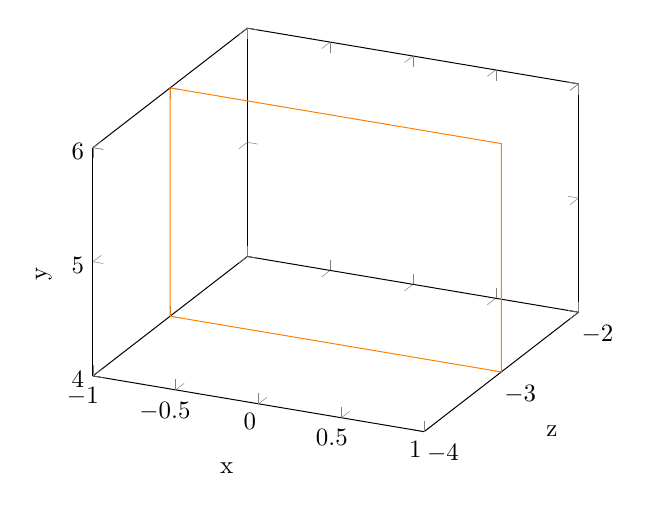
\begin{tikzpicture}[xscale=0.9,yscale=0.9]
    \begin{axis}[
        % nodes near coords={(\coordindex)},
        xmax=1,xmin=-1,ymax=-2,ymin=-4,zmin=4,zmax=6,
        xlabel={x},
        ylabel={z},
        zlabel = {y}]
	\addplot3 [orange] coordinates {(1,-3,4)(1,-3,6)(-1,-3,6)(-1,-3,4)(1,-3,4) };
    \end{axis}
\end{tikzpicture} \hspace{2cm}
\begin{tikzpicture}[xscale=0.9,yscale=0.9]
    \begin{axis}[
        % nodes near coords={(\coordindex)},
        xlabel={$x$},
        ylabel={$y$}]
	\addplot [black] coordinates {(1,4)(1,6)(-1,6)(-1,4)(1,4) };
    \end{axis}
\end{tikzpicture}

}

\end{document}